% $Id: introduction.tex 87303 2016-02-08 13:44:29Z lafferty $

\section{Introduction}
\label{sec:Introduction}

The $s\to d$ decay processes (see \figref{fig:diagram}) have the strongest CKM suppression factor of all quark transitions.
Hence, they are particularly sensitive to sources of flavour violation different from those of the
Standard Model (SM). Indeed, flavour violation can induce detectable effects at accessible energy in flavour-changing processes
even if the scale of the new dynamics is heavy and well above their direct production at accelerators.
Among these transitions, the decay \Klpizmm has been shown to be sensitive to, for example, models
with extra dimensions~\cite{Bauer:2009cf}. However, the potential for this decay to constrain scenarios
beyond the Standard Model is limited by the large SM uncertainty on its branching fraction prediction~\cite{Bauer:2009cf},%~\cite{D'Ambrosio:1998yj} 
\begin{equation}
{{\cal B}({\PKzL}\to\Pgpz\APmuon\Pmuon)_{\rm SM} = \{1.4\pm0.3; 0.9\pm0.2\}\times 10^{-11}.}
\end{equation}
The two numbers in the brackets correspond to two theoretical solutions, 
depending on whether constructive or destructive interference between the contributing waves is present.
The reason for the large theoretical uncertainty on ${\cal B}({\PKzL}\to\Pgpz\APmuon\Pmuon)_{\rm SM}$ is the limited
precision on the chiral-perturbation-theory parameter $|a_S|$. An improved measurement of \BRof\Kspizmm will reduce this uncertainty.
%\noindent compared to the experimental value:
%\begin{equation}
%{\cal B}({\PKzL}\to\Pgpz\APmuon\Pmuon)_{\rm exp} < 3.8\times 10^{-10}
%\end{equation}
% which is due to the limited experimental precision on \BRof\Kspizmm. 
The most precise measurement of \BRof\Kspizmm was performed by the NA48 experiment at CERN~\cite{NA48}, which obtained
\begin{equation}
{\cal B}({\PKzS}\to\Pgpz\APmuon\Pmuon) = (2.9^{+1.5}_{-1.2}\text{(stat)}\pm0.2\text{(syst)})\times10^{-9}.
\label{eq:NA48}
\end{equation}

\begin{figure} [htb!]
\begin{center}
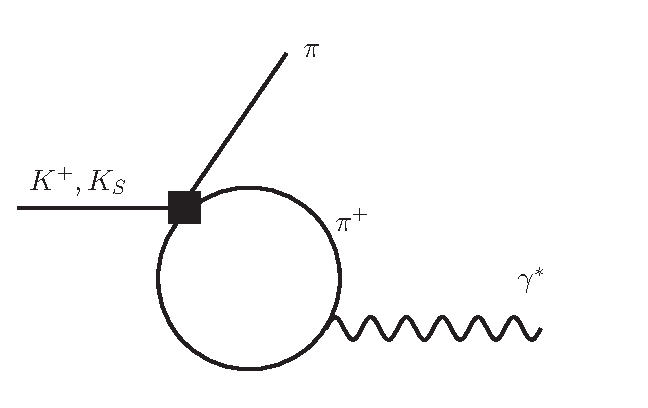
\includegraphics[scale=0.5]{figs/Cirigliano_fig17.pdf} %ks_pi0mumu.pdf}
\caption{Feynman diagram of the process \Kzpizmm. \label{fig:diagram}}
\end{center}
\end{figure}

The LHCb experiment~\cite{LHCbDet} has demonstrated very good performance in the search for rare leptonic \KS decays~\cite{Ksmm}. In this note, we evaluate the potential
sensitivity of LHCb to \BRof\Kspizmm considering the data to be collected with the LHCb detector before and after its upgrade in 2018.
 
This document is organized as follows: in~\secref{sec:strategy}, the analysis strategy is summarized; in \secref{sec:selection}, details on the signal reconstruction and selection are given;
in \secref{sec:background}, the study on the expected background sources is presented; in \secref{sec:fit}, the likelihood fit is described; in~\secref{sec:sensitivity}, the sensitivity to
\BRof\Kspizmm is reported and finally, conclusions are drawn in~\secref{sec:conclusions}.
